%\documentclass{spie}
%\usepackage[pdftex]{graphicx}
%\usepackage{psfig}
%\begin{document}

\chapter{Mast Bending report}
The bending of the mast due to the sun/shade is a very important effect which needs to be implemented in NuSIM. Simulations of the mast bend are available for a handful of solar angles. These are given as deviations in the location of the optical axis on the focal plane, and assuming that the mast will arc as it bends, we decompose the transformation between the two benched due to the mast, as a rotation and translation. We then generate a database from these values and input them into NuSIM.

\section{Mast bend model and database generation}

\begin{figure}[tb]
\begin{center}
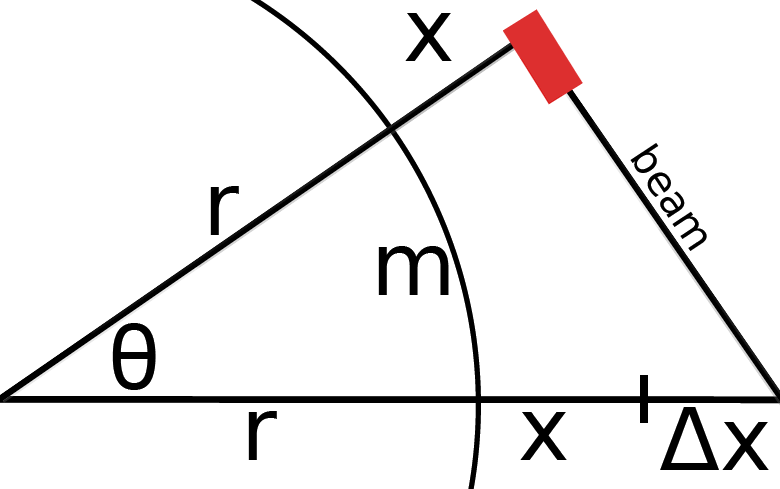
\includegraphics[width=0.5\textwidth]{images/mast_bending_model.png}
\caption{Mast model.}
\label{mastmodel}
\end{center}
\end{figure}

\subsection{Modeling the Mast as an Arc}

The document ``Thermal\_Distortion\_2\_for\_JPL.xlsx" details the effects on the mast under the thermal effects of sunlight. In particular, it provides $x$ and $y$ offsets of the optical axis impingement on the focal plane, as well as $\theta_z$, the twisting of the mast itself around the z-axis. 

A few assumptions had to be made in order to decompose the mast bend into a rotation quaternion, $Q_{fbob}$ and a translation, $T_{fbob}$ which together create $R_{fbob}$:

\begin{itemize}
    \item The twist in the mast is small enough that its effect on the bend of the mast is not worth calculating, which is to say it can be interpreted as one of the benches at either end having been rotated about the mast.
    \item The mast bend in $x$ and $y$ dimensions can be interpreted as separate arcs 
    \item The optical axis from the optics modules are exactly parallel to the mast when there is no bend.
    \item Over these small angles, second order approximations of cosine are acceptable. 
\end{itemize}

Figure \ref{mastmodel} illustrates the mast model geometry. The coordinate system in this image and for the remainder of this document is aligned such that $z$ points up, and $y$ points into the paper. The mast is represented by the arc labelled 'm' , which has length $m= \theta r$. The red square represents the optic and the vertices labelled 'beam' the optical axis of the optic. In the case of no bend, where $\theta=0$, the optical axis would intersect at r+x. Because of the mast bending, the axis now intersects at r+x+$\Delta x$. In addition, the mast also rotates around its own axis by $\theta_z$ not illustrated in the figure.

First, to align the coordinate of the mast with the focal plane properly, the distortion of $\Delta x$ and $\Delta y$ must be modified by $\theta_z$:
\begin{eqnarray}
r = \sqrt{x^2+y^2}\\
\psi = \arctan \left(\frac{\Delta x}{\Delta y}\right)\\
\Delta Y = r \sin (\psi-\theta_z)\\
\Delta X = r \cos (\psi-\theta_z)\\
\end{eqnarray}

Let $m$ be the length of the mast itself. The arc angle, $\theta$, and the arc radius, $r$, can be determined as follows:

The mast is essentially an arc (of radius $r$) with the optics module extending out by a distance $x$. The angle, $\theta$, of the arc can be found from:
\[
\cos \left( \theta \right) = \frac{r+x}{r+x+\Delta x}
\]
A general rule of arcs is:
\[
m = \theta r
\]
So:
\[
\cos \left( \theta \right) = \frac{\frac{m}{\theta}+x}{\frac{m}{\theta}+x+\Delta x}
\]
This is not solvable analytically, so here we shift to a second order approximation of $\cos$, which should be accurate for these small angles:
\[
1-\frac{\theta^2}{2} \approx \frac{\frac{m}{\theta}+x}{\frac{m}{\theta}+x+\Delta x}
\]
For which the solutions for $\theta$ are:
\[
\theta = \frac{-m \pm \sqrt{m^2+8x\Delta x + 8{\Delta x}^2}}{2 \left( x + \Delta x \right)}
\]
Given that when $\Delta x = 0$, $\theta = 0$, the correct solution is:
\[
\theta = \frac{-m + \sqrt{m^2+8x\Delta x + 8{\Delta x}^2}}{2 \left( x + \Delta x \right)}
\]
Which does indeed grow as expected as $\Delta x$ grows, so it seems a reasonable solution. 


Given $\theta$, and $r = \frac{m}{\theta}$, It should be clear that the optics bench will move by $r\left(1-\cos\left(\theta\right)\right)$ along the $x$ axis and $r\sin\left(\theta\right)-m$ along the $z$ axis. 

The calculated bend of the mast by a displacement $\Delta x$, is a rotation around the y-axis and vice versa.

\subsection{Database creation}

\begin{figure}[tb]
\begin{center}
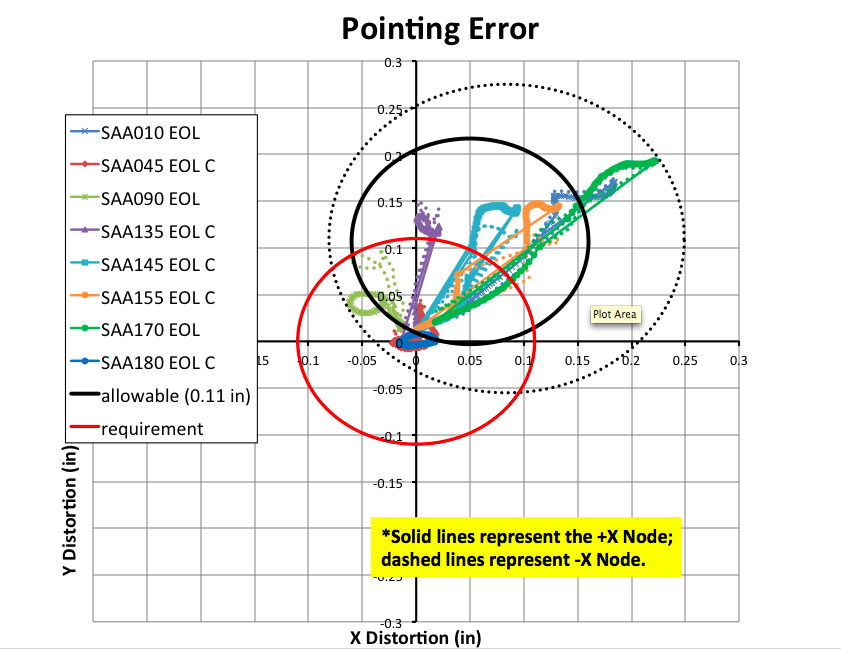
\includegraphics[width=0.7\textwidth]{images/mastdb.png}
\caption{Simulated Thermal scenarios.}
\label{mastdb}
\end{center}
\end{figure}

We have converted three thermal scenarios into databases: SAA90, SAA135 and SAA170. Figure \ref{mastdb} shows the mast distortions of several solar angles, and SAA90 is considered a 'good case', SAA135 a "conservative case', and SAA170 a 'very bad case'. SAA90 and SAA135 have distortions within the allowed range, while SAA170 is slightly larger than the allowable distortion.

Figures \ref{saa90sim}, \ref{saa135sim} and \ref{saa170sim} show the footprint of the optical axis on the focal plane for the three thermal scenarios. The red diamonds are the simulated thermal distortions ($\Delta x, \Delta y$) which are used in the formulas presented above to derive the transformation between the benches, $R_{fbob}$. The black stars are the result of ray-tracing the optical axis using the obtained transformation $R_{fbob}$.  The agreement is good and tolerable considering the approximations that went into the derivation, and we consider this a good enough representation of the mast bend for use in NuSIM.

\begin{figure}[tb]
\begin{center}
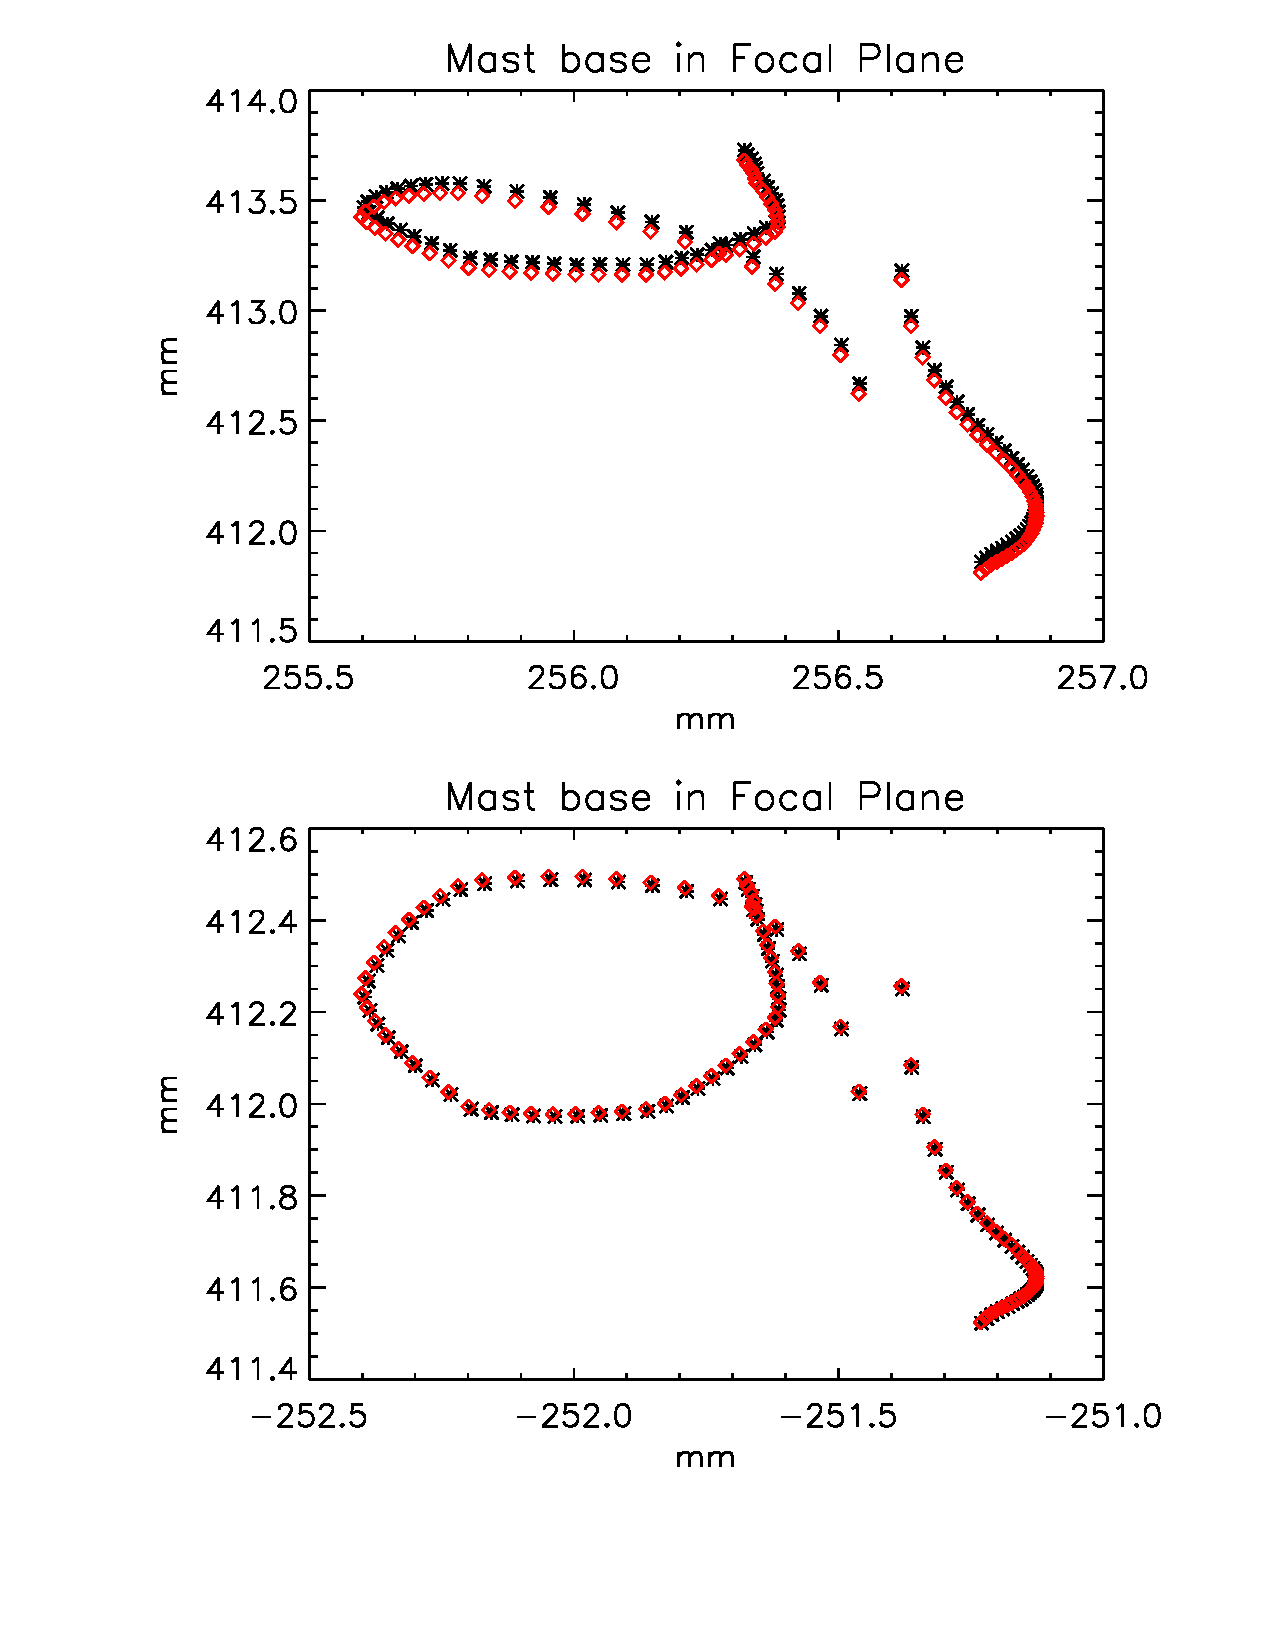
\includegraphics[width=0.8\textwidth]{images/saa90mastbend1.pdf}
\caption{SAA90 thermal mast bend distortions. Coordinates are in focal plane. Top: distortion footprint of module 1. Bottom: distortion footprint of module 2. Black stars are the ray-traced intersections of the optical axis using the transformation of the benches obtained from the thermal mast bend database which are plotted in red diamonds.}
\label{saa90sim}
\end{center}
\end{figure}

\begin{figure}[tb]
\begin{center}
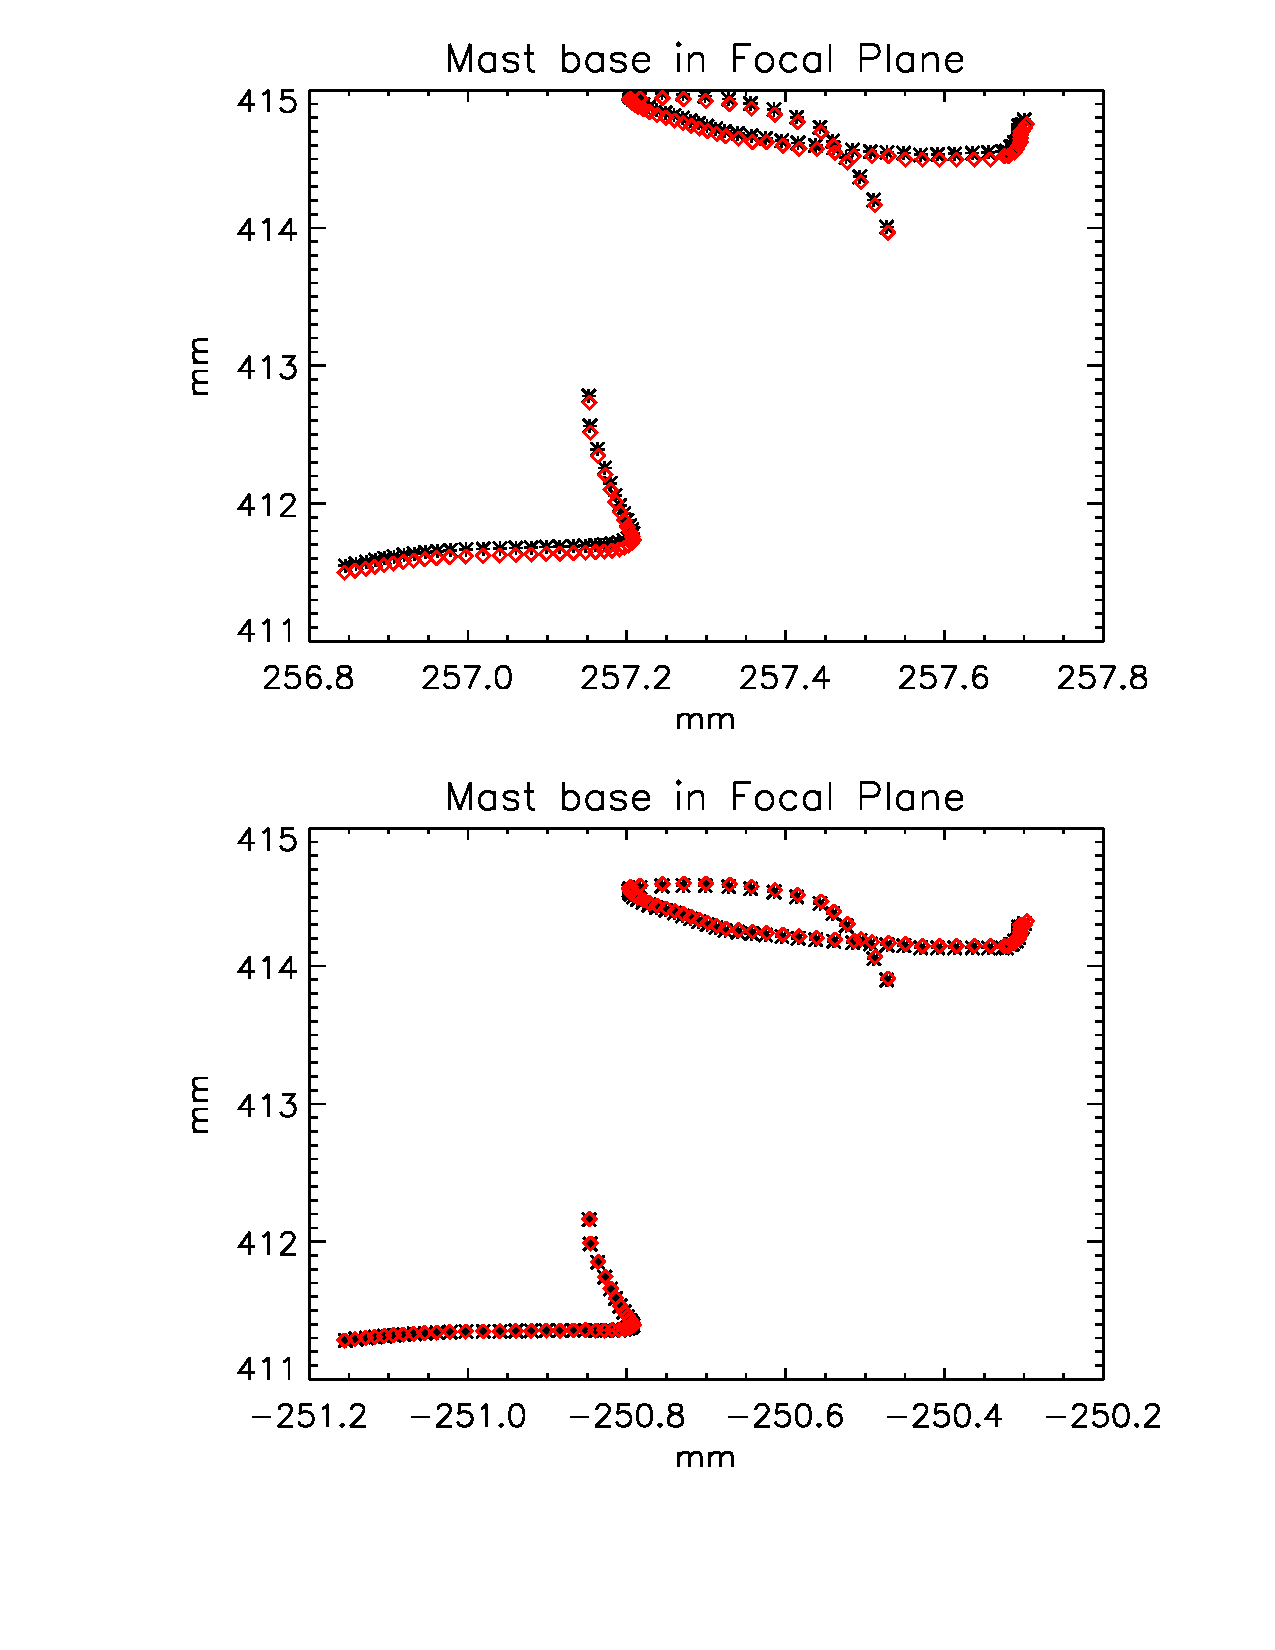
\includegraphics[width=0.8\textwidth]{images/saa135mastbend1.pdf}
\caption{SAA135 thermal mast bend distortions. Coordinates are in focal plane. Top: distortion footprint of module 1. Bottom: distortion footprint of module 2. Black stars are the ray-traced intersections of the optical axis using the transformation of the benches obtained from the thermal mast bend database which are plotted in red diamonds.}
\label{saa135sim}
\end{center}
\end{figure}

\begin{figure}[tb]
\begin{center}
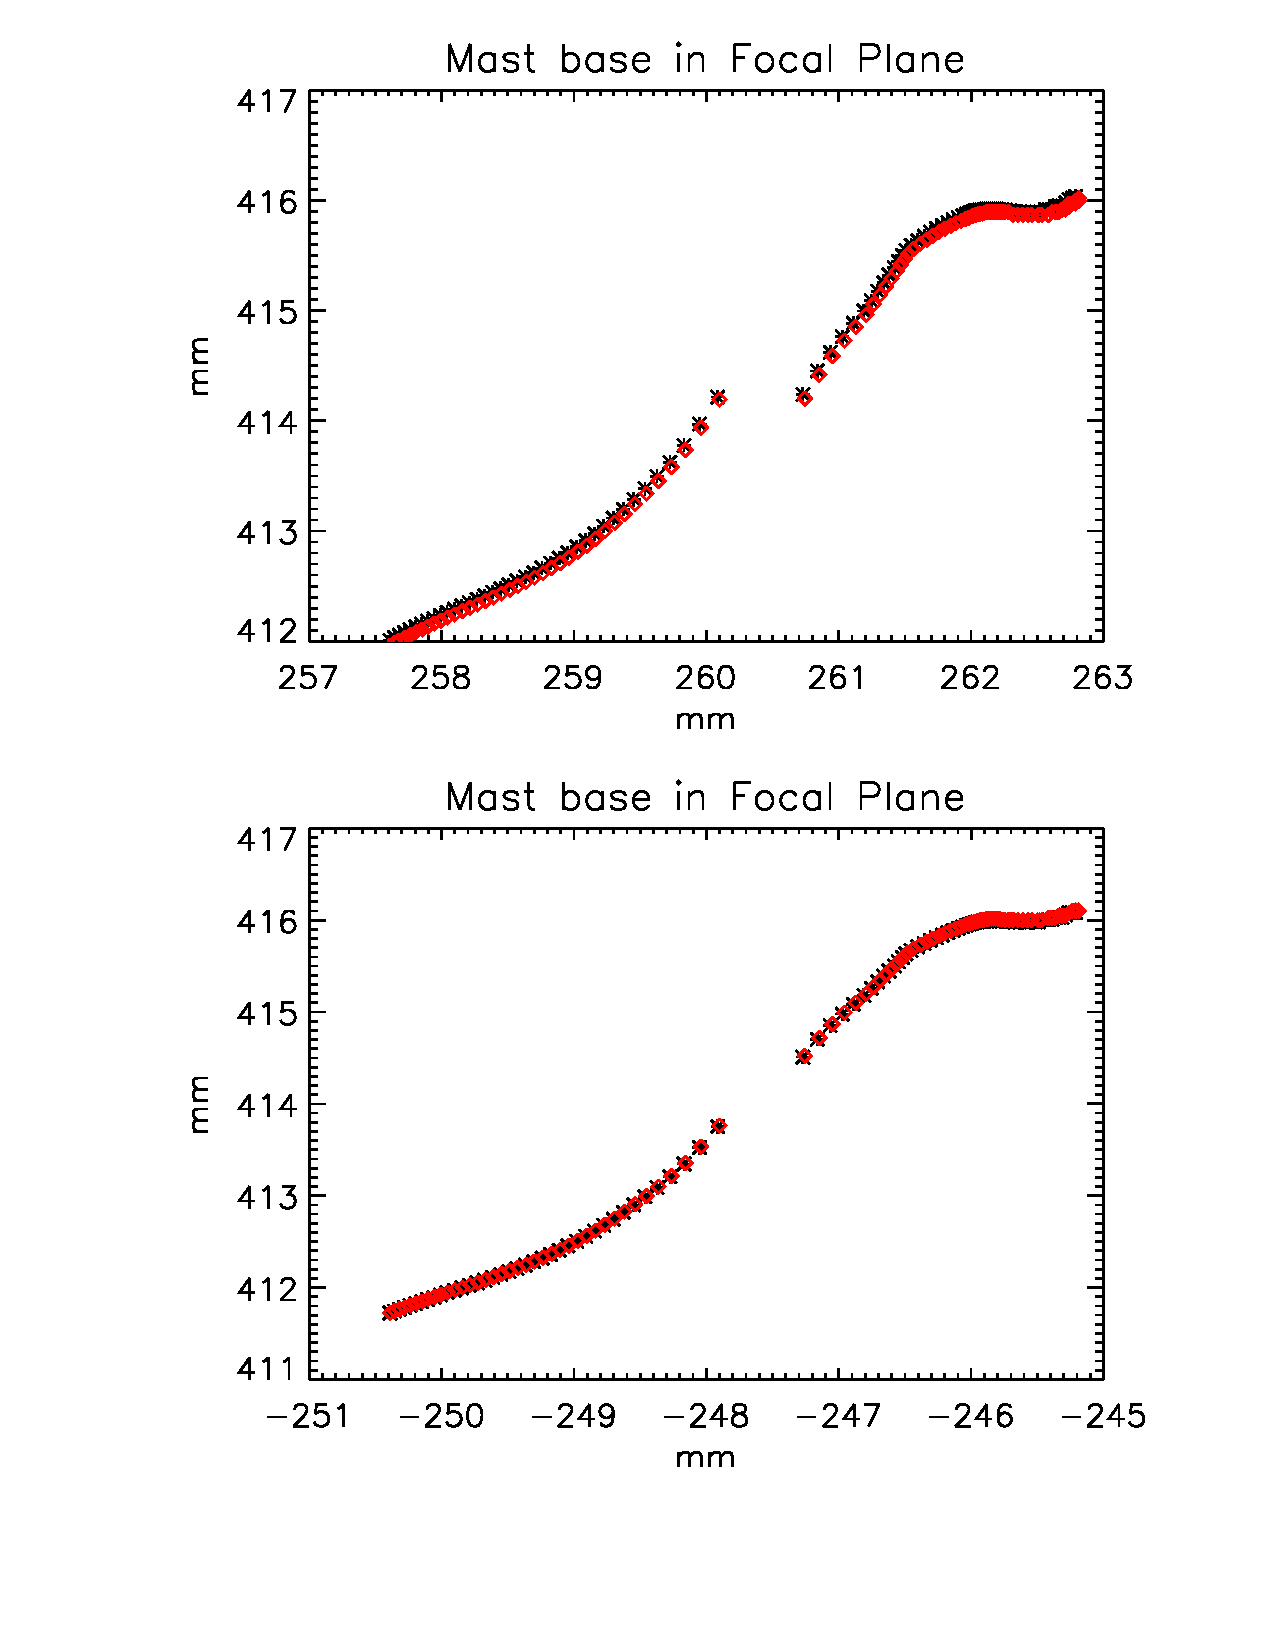
\includegraphics[width=0.8\textwidth]{images/saa170mastbend1.pdf}
\caption{SAA170 thermal mast bend distortions. Coordinates are in focal plane. Top: distortion footprint of module 1. Bottom: distortion footprint of module 2. Black stars are the ray-traced intersections of the optical axis using the transformation of the benches obtained from the thermal mast bend database which are plotted in red diamonds.}
\label{saa170sim}
\end{center}
\end{figure}

\section{NuSIM results}

The challenge for NuSIM is to reconstruct the pointing when using the mast bending databases as input. The NuSIM aspect reconstruction is insensitive to relative bend of the two benches, and it is therefore important to discover how well a pointing can be reconstructed.

Figures \ref{saa90nusim}, \ref{saa135nusim} and \ref{saa170nusim} show the reconstructed Ra and Dec of the pointing. In running this test we used perfect optics without scattering included or any error terms in the sensors. The error, as can be seen, is very small, and in all cases less than the width of a pixel (12''). 

\begin{figure}[tb]
\begin{center}
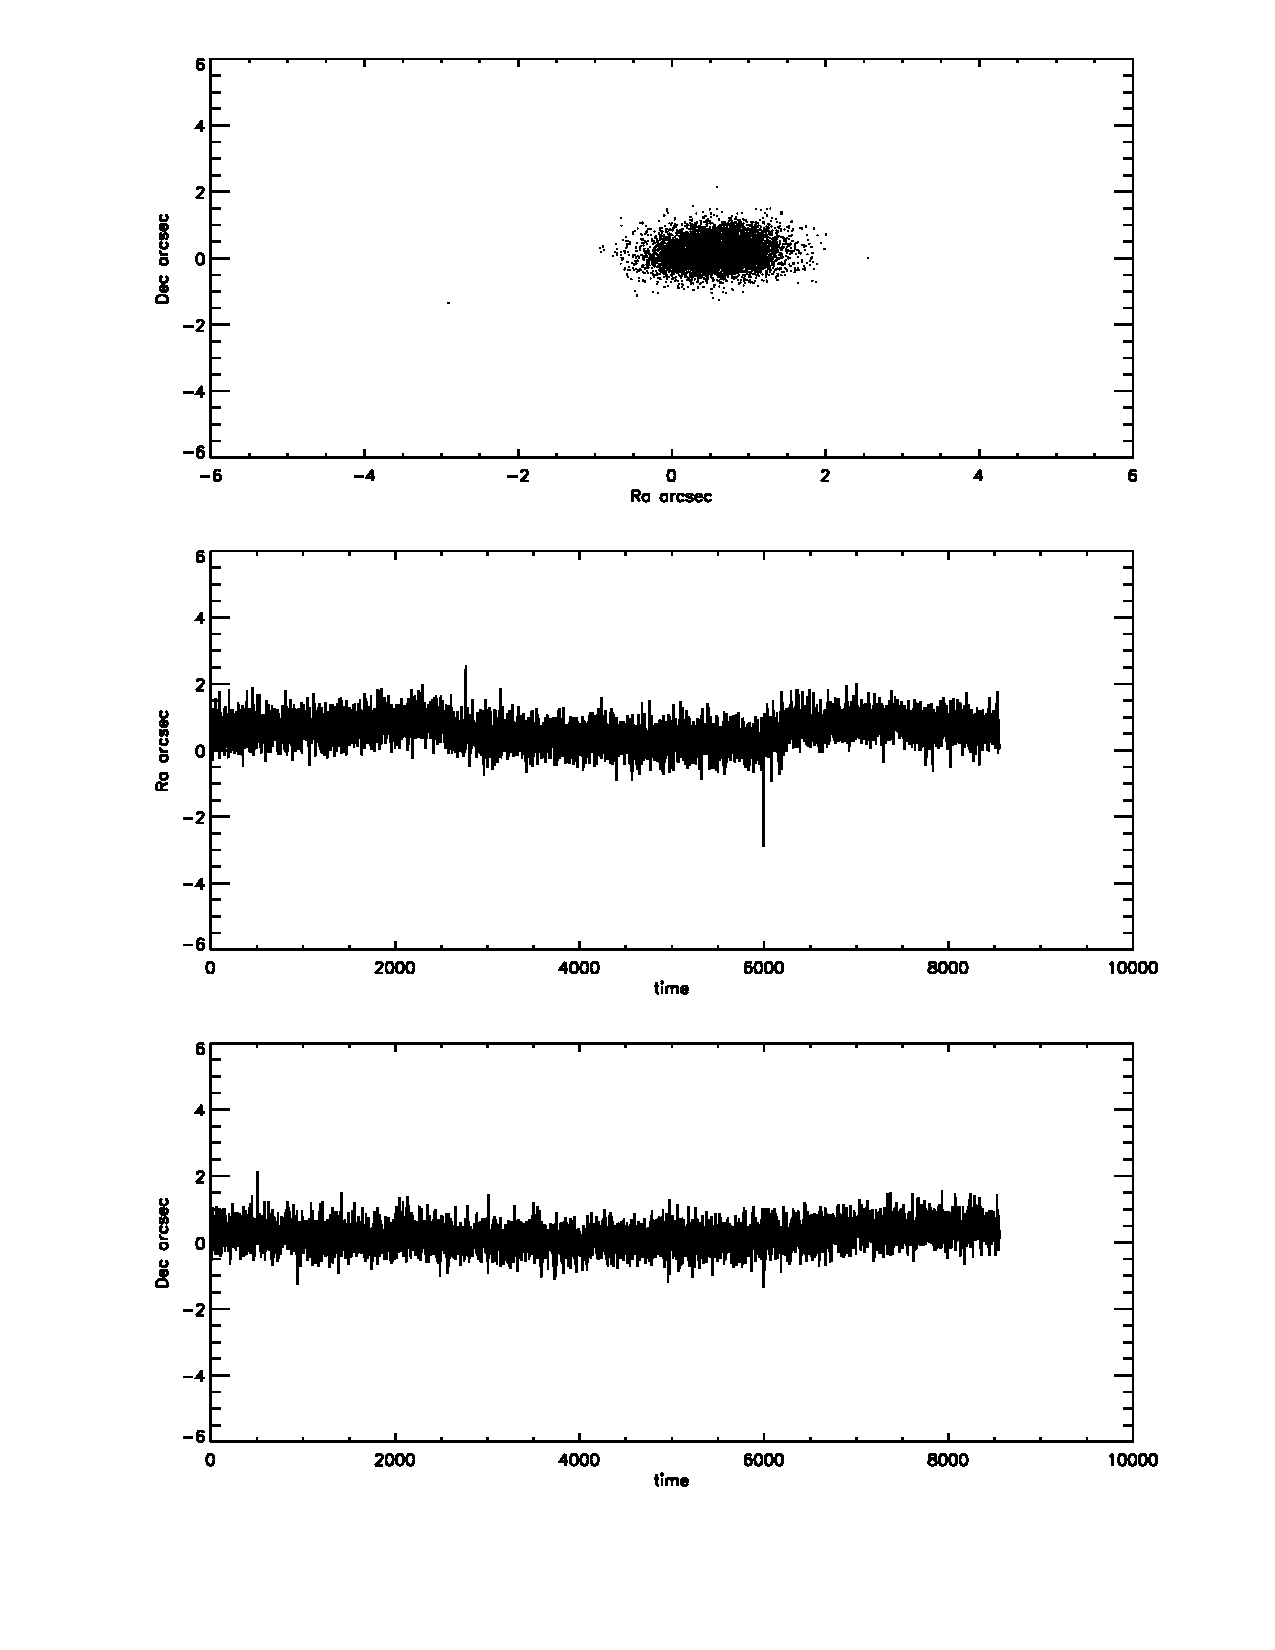
\includegraphics[width=0.8\textwidth]{images/saa90.pdf}
\caption{Aspect reconstruction of SAA90 thermal mast bend. Top: Ra and Dec error. Source pointing is at RA,DEC=0,0. Middle: Ra error as a function of time. Bottom: Declination error as a function of time. }
\label{saa90nusim}
\end{center}
\end{figure}

\begin{figure}[tb]
\begin{center}
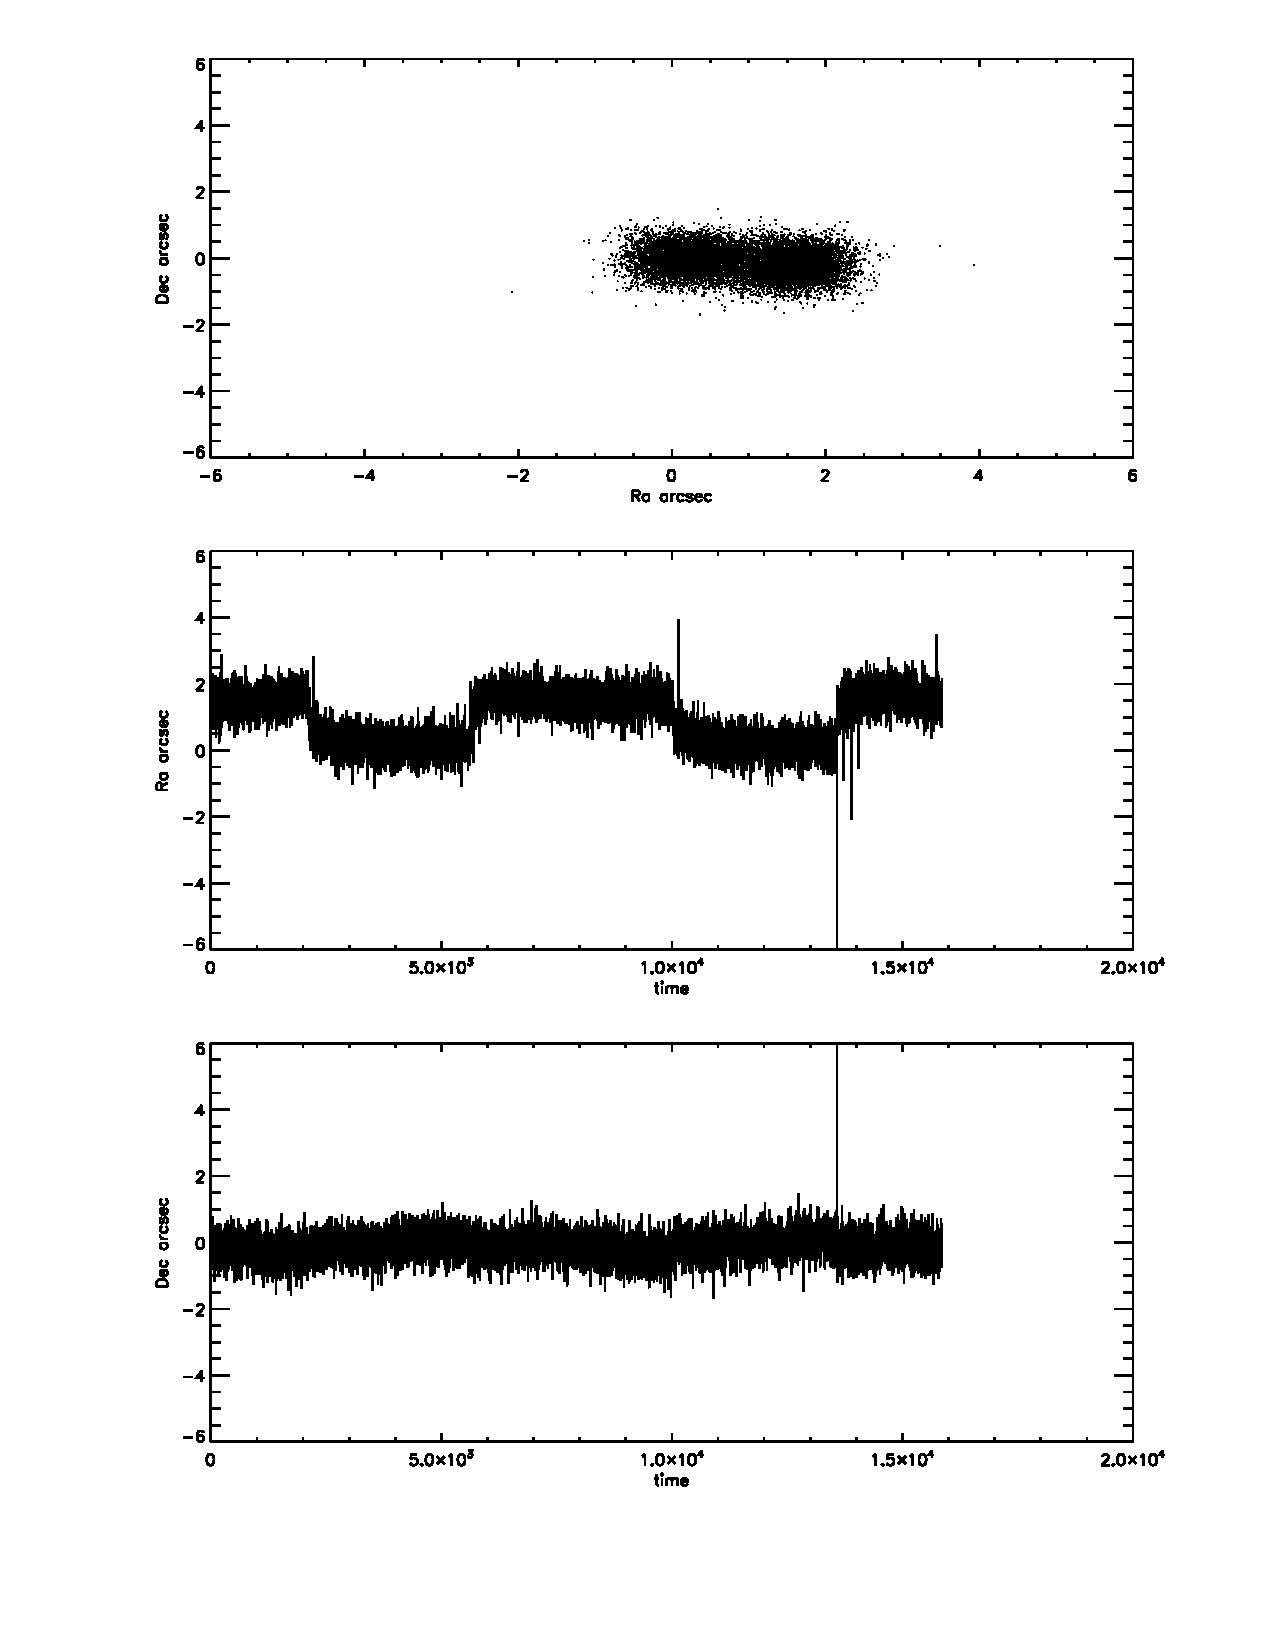
\includegraphics[width=0.8\textwidth]{images/saa135.pdf}
\caption{Aspect reconstruction of SAA135 thermal mast bend. Top: Ra and Dec error. Source pointing is at RA,DEC=0,0. Middle: Ra error as a function of time. Bottom: Declination error as a function of time. }
\label{saa135nusim}
\end{center}
\end{figure}

\begin{figure}[tb]
\begin{center}
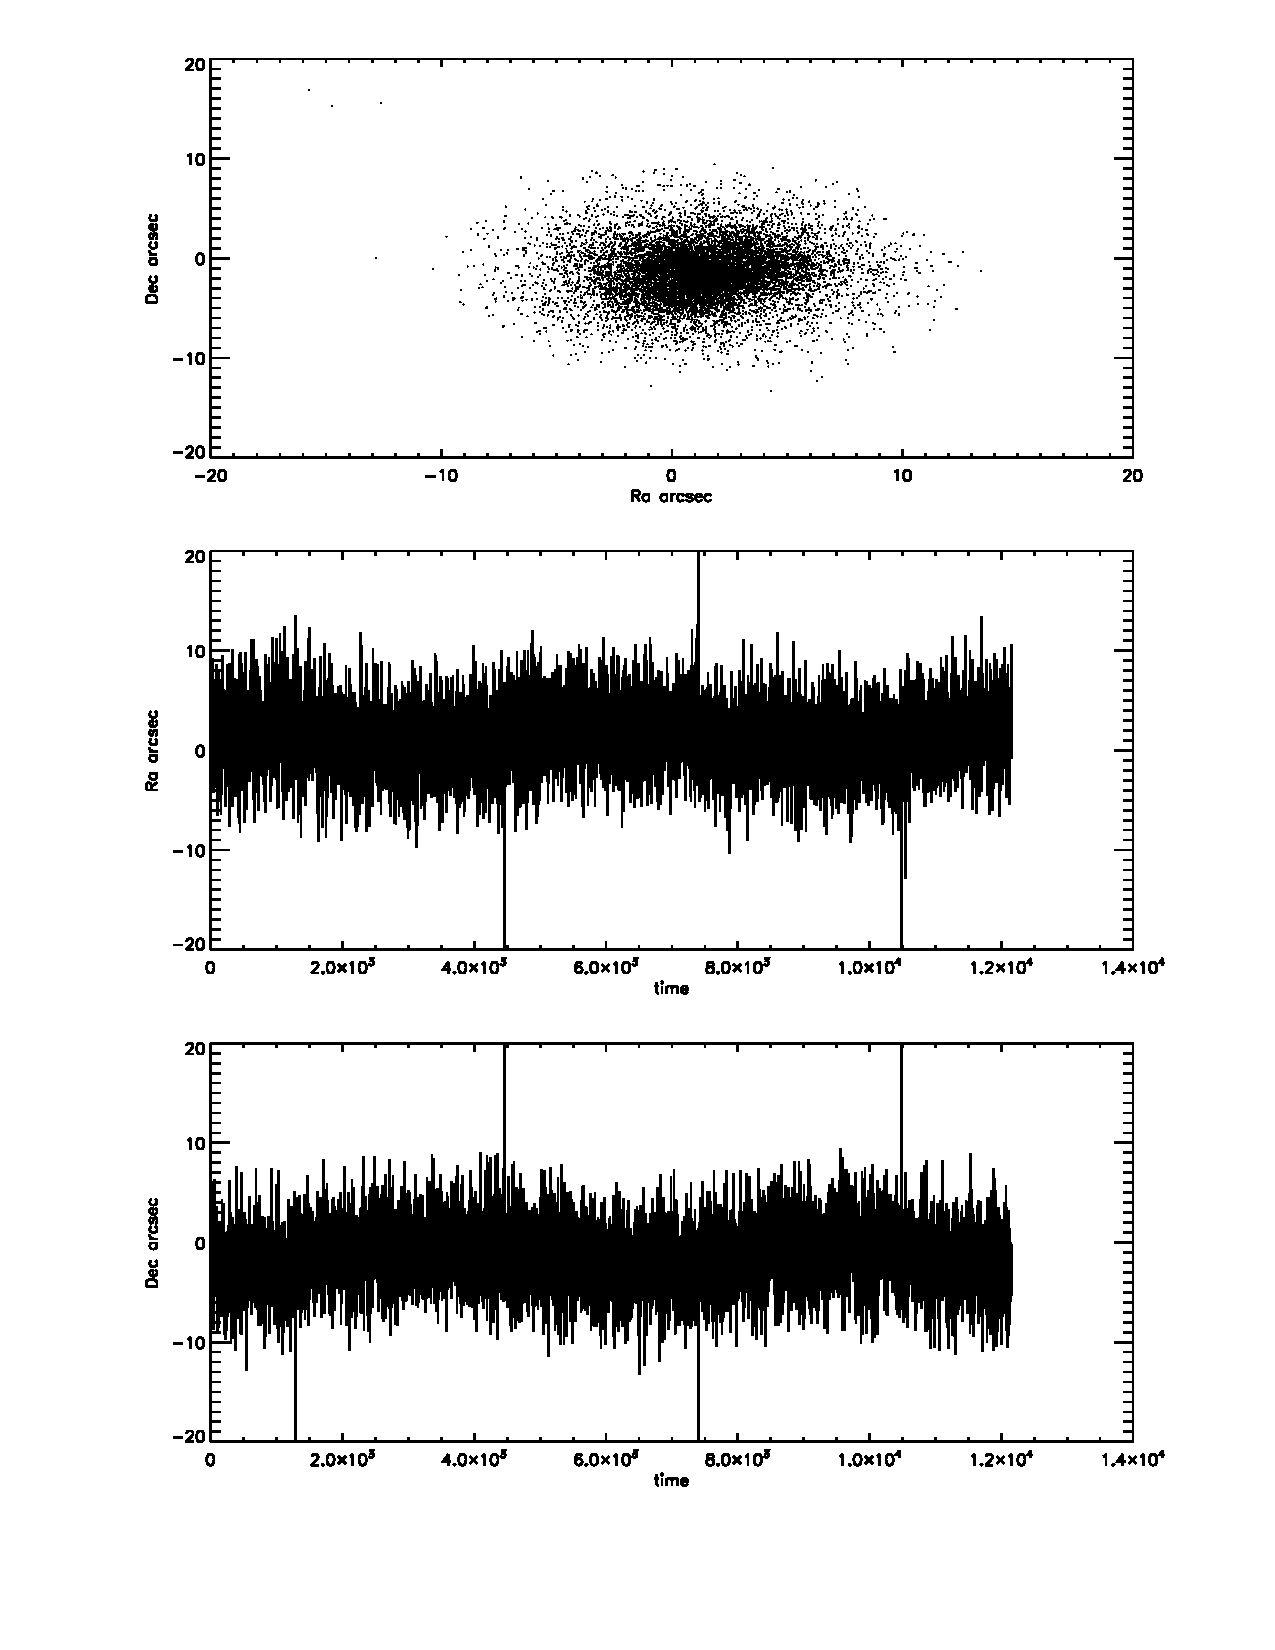
\includegraphics[width=0.8\textwidth]{images/saa170.pdf}
\caption{Aspect reconstruction of SAA170 thermal mast bend. Top: Ra and Dec error. Source pointing is at RA,DEC=0,0. Middle: Ra error as a function of time. Bottom: Declination error as a function of time. }
\label{saa170nusim}
\end{center}
\end{figure}

\section{Comparison with external code}

Even though the error is small it is important to understand its source and so we compared the reconstructed transformation, $R_{fbob}$, which lacks information about rotations around x- and y-axis, with the original, $R_{true}$. Figures \ref{saa90re}, \ref{saa135re} and \ref{saa170re} show the optical axis ray-traced with the true, $R_{true}$, in red diamonds and reconstructed, $R_{recon}$, in black dots. The error here is due to the fact that the reconstructed transformation only has a rotation around the z-axis, and has replaced the rotations around x-, y-axis with translations. The error in the pointing is thus due to the slight distortion in the footprint which can now be seen to be less than a pixel width (0.6mm).

\begin{figure}[tb]
\begin{center}
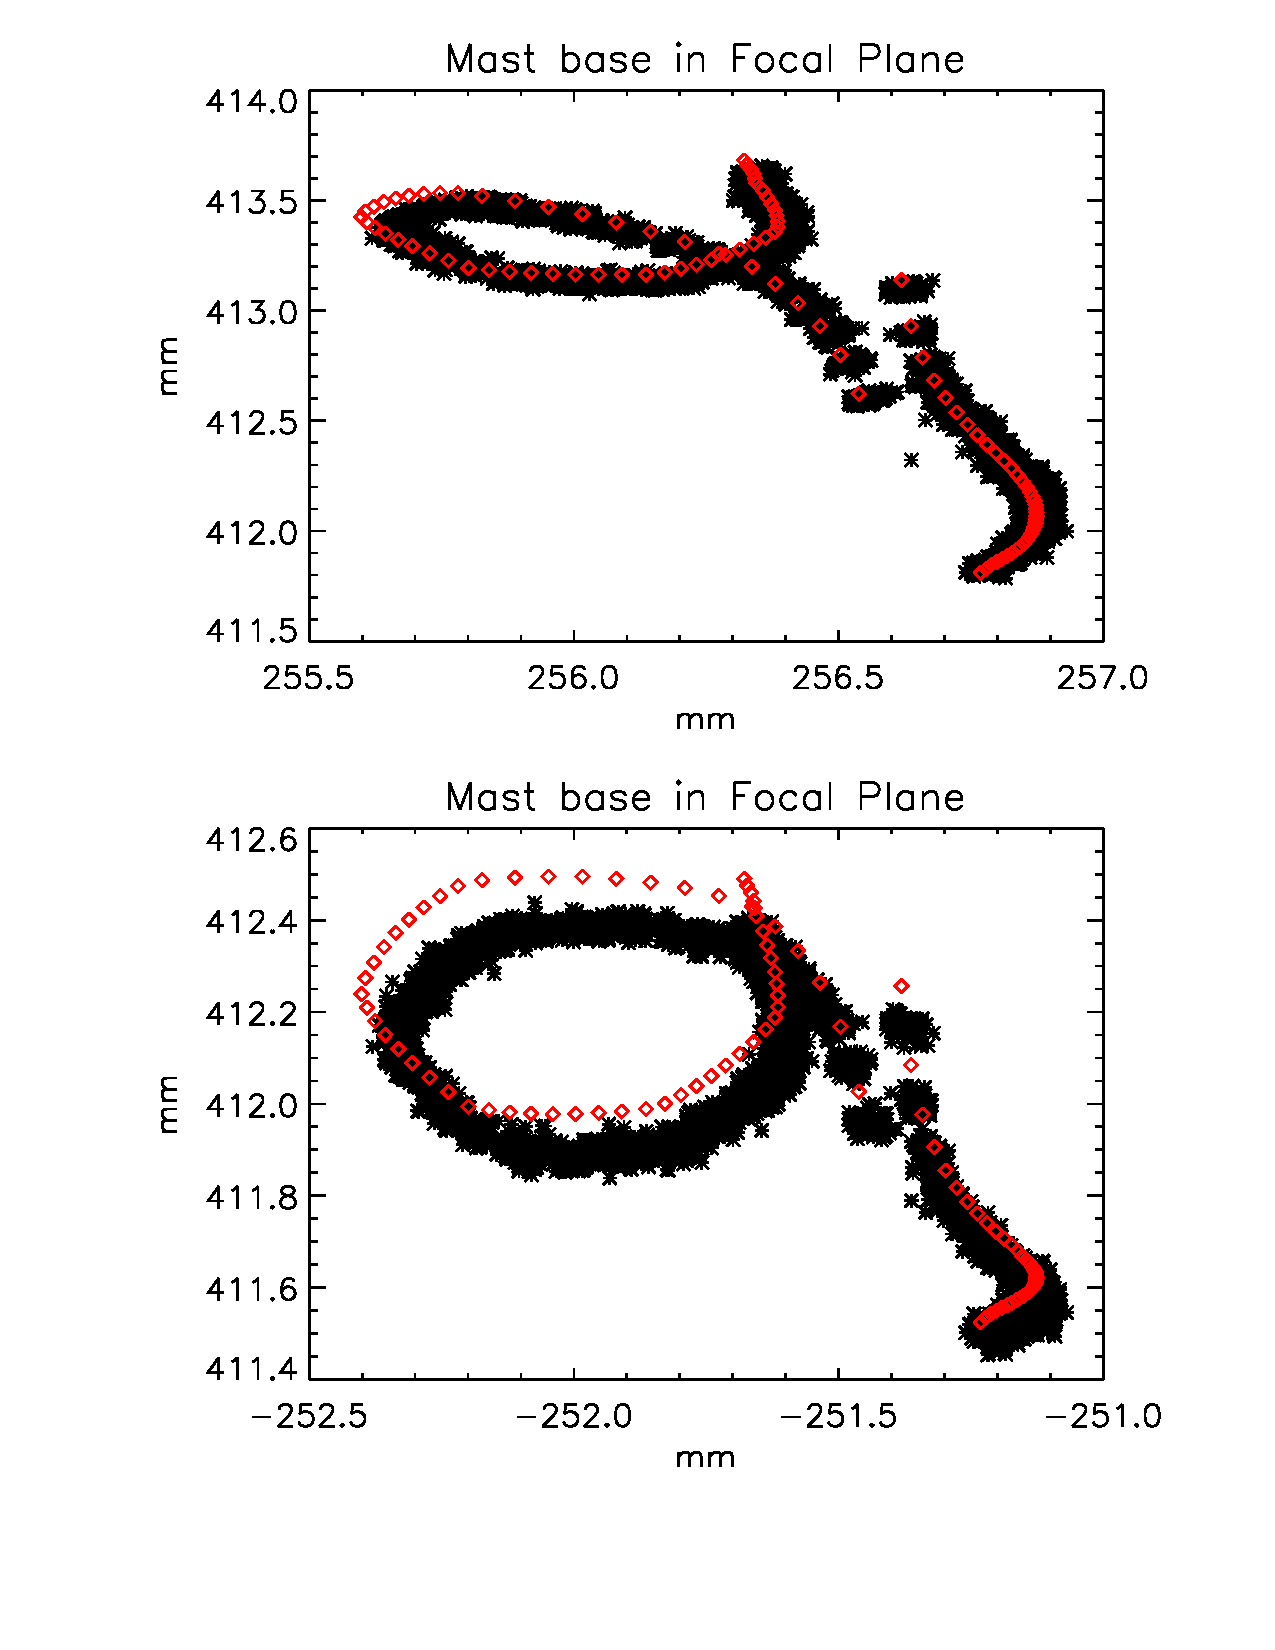
\includegraphics[width=0.8\textwidth]{images/saa90mastbend2.pdf}
\caption{SAA90 thermal mast bend distortions. Coordinates are in focal plane. Top: distortion footprint of module 1. Bottom: distortion footprint of module 2. Black stars are the ray-traced intersections of the optical axis using the reconstructed transformation of the benches obtained from the NuSIM. The original transformation is plotted in red diamonds.}
\label{saa90re}
\end{center}
\end{figure}

\begin{figure}[tb]
\begin{center}
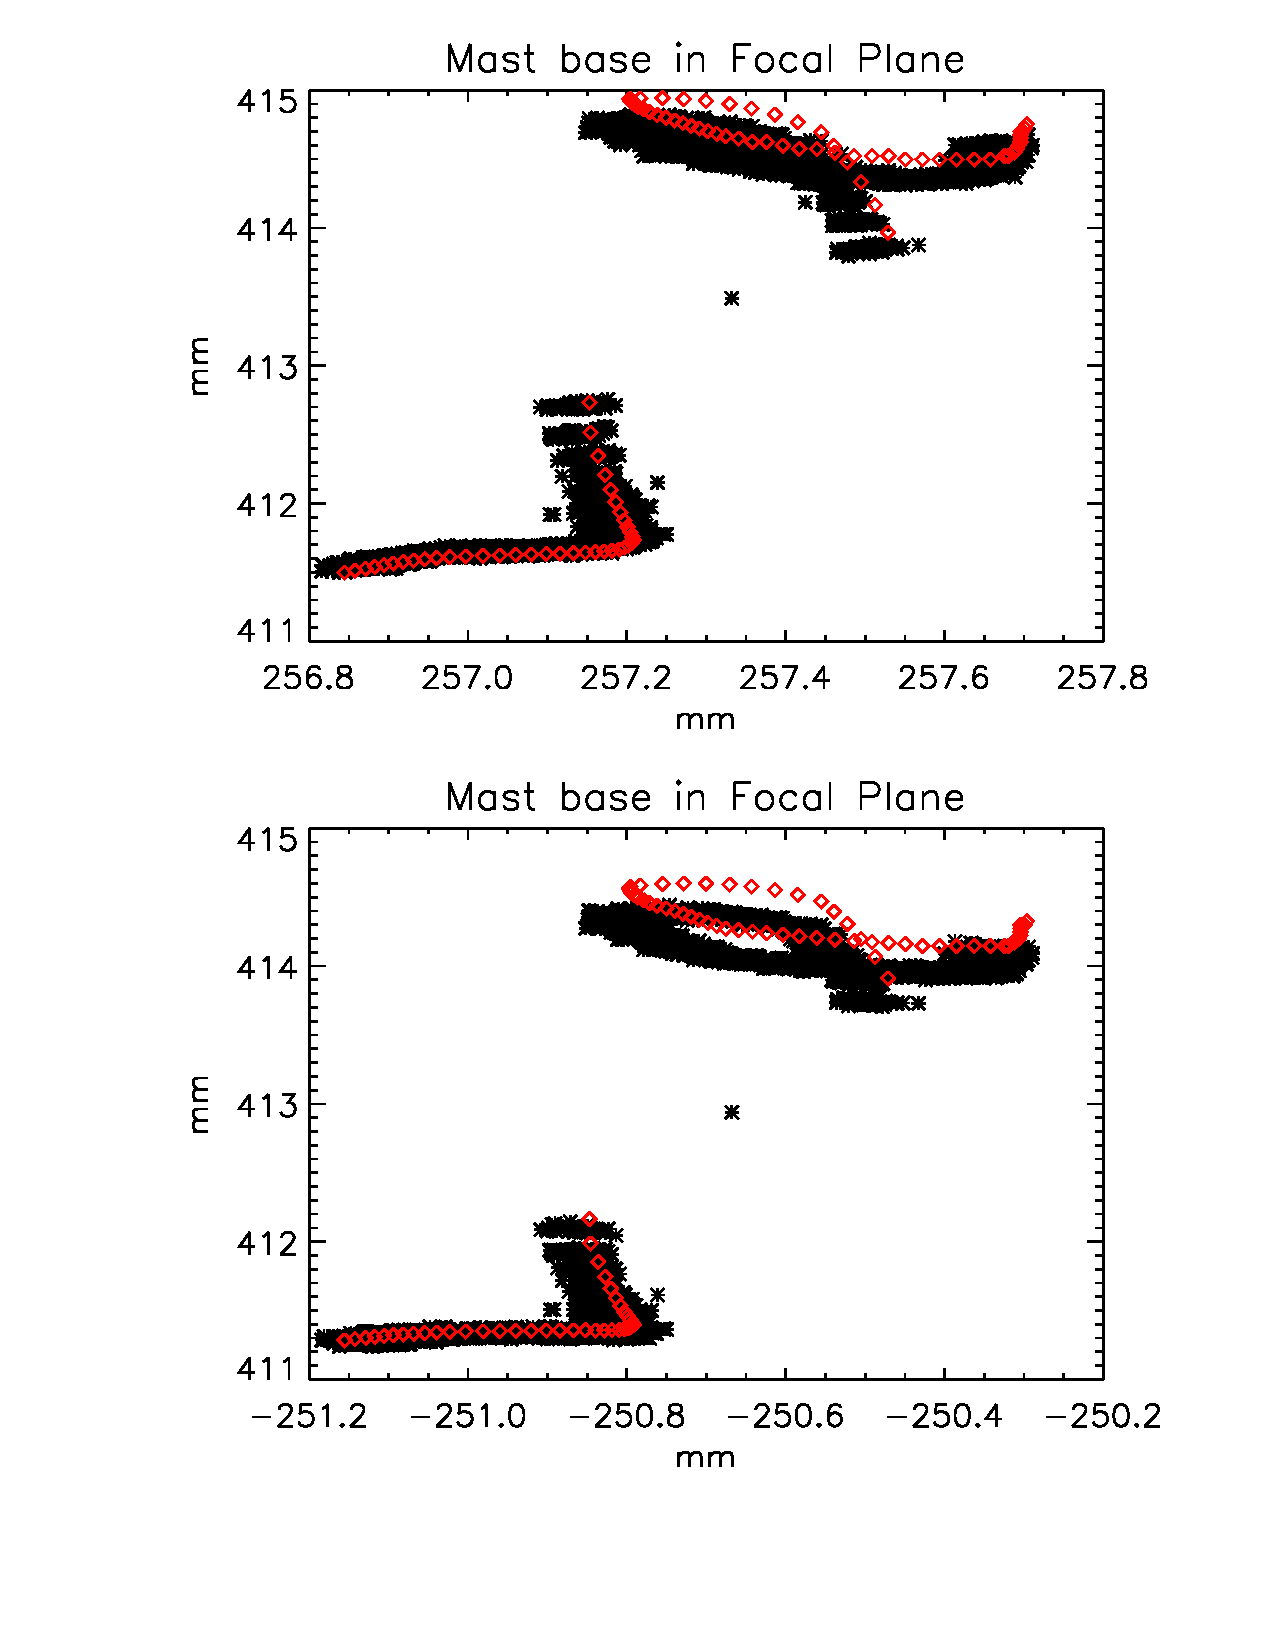
\includegraphics[width=0.8\textwidth]{images/saa135mastbend2.pdf}
\caption{SAA135 thermal mast bend distortions. Coordinates are in focal plane. Top: distortion footprint of module 1. Bottom: distortion footprint of module 2. Black stars are the ray-traced intersections of the optical axis using the reconstructed transformation of the benches obtained from the NuSIM. The original transformation is plotted in red diamonds.}
\label{saa135re}
\end{center}
\end{figure}

\begin{figure}[tb]
\begin{center}
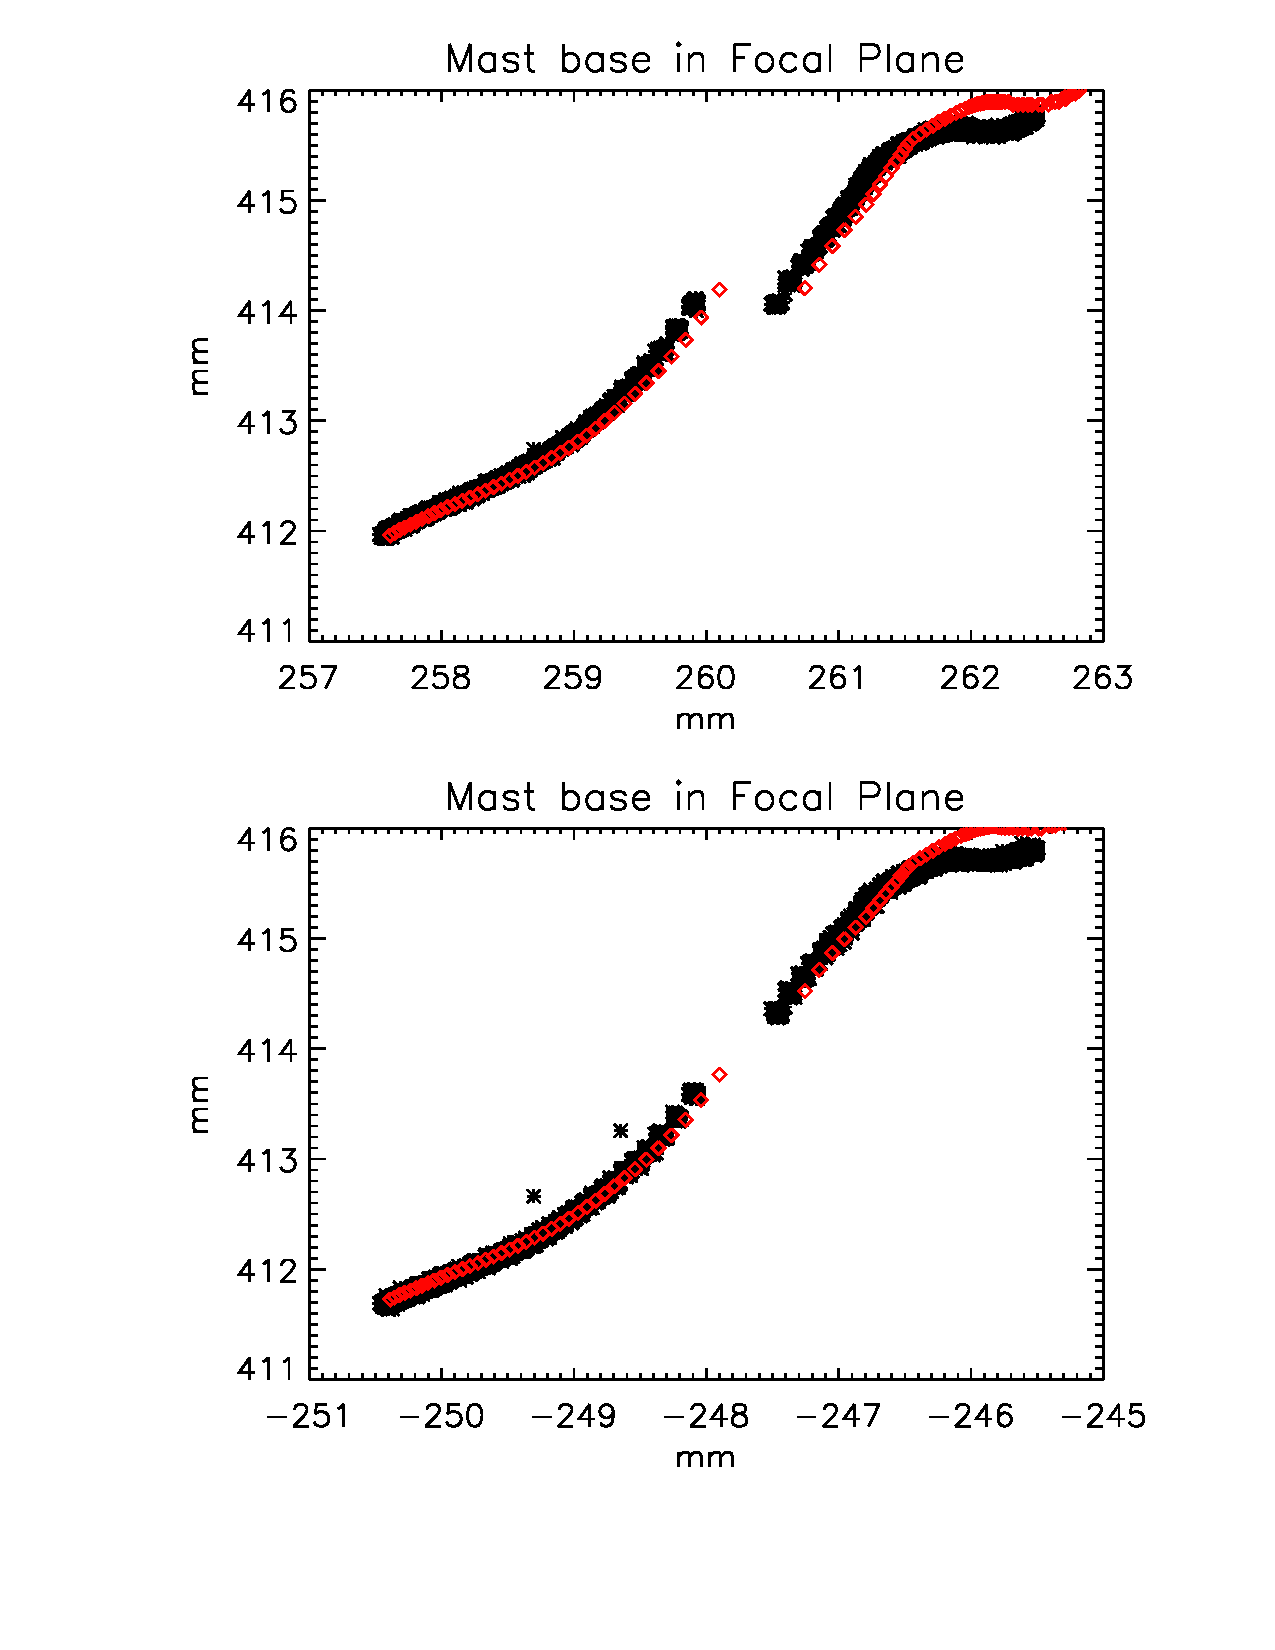
\includegraphics[width=0.8\textwidth]{images/saa170mastbend2.pdf}
\caption{SAA170 thermal mast bend distortions. Coordinates are in focal plane. Top: distortion footprint of module 1. Bottom: distortion footprint of module 2. Black stars are the ray-traced intersections of the optical axis using the reconstructed transformation of the benches obtained from the NuSIM. The original transformation is plotted in red diamonds.}
\label{saa170re}
\end{center}
\end{figure}

\section{Conclusion}
The NuSIM aspect reconstruction can not perfectly reconstruct the mast pointing due to the fact that it cannot tell a rotation of the plane from a translation of the plane. However, the errors are very small and within the budget. The mast bend databases are therefore considered valid and the aspect reconstruction of the mast movement understood, acceptable and thus verified.

%\end{document}

